\chapter{Data Analysis} \label{ch:analysis}
This thesis details the method of transverse energy analysis through the use of $p_{T}$ spectra from the STAR BES data. As described in section \ref{subsec:tracking_STAR}, the TPCs and TOF detectors in STAR can identify particles as well as their trajectories and ultimately measure their multiplicity distributions with respect to the momenta. The availabe distributions were extrapolated to calculate the transverse energies and charged particle multiplicities. Details follow.

\subsection{STAR $p_{T}$ spectra}
\citet{PhysRevC.96.044904} reports the results for the $p_{T}$ spectra for six different identified hadrons, $\pi^+$, $\pi^-$, $K^+$, $K^-$, $p$, and $\bar{p}$, from the STAR experiment. The spectra come from $\sqrt{s_{NN}}$ = 7.7, 11.5, and 39 GeV Au+Au collisions data taken in the year 2010, and from $\sqrt{s_{NN}}$ = 19.6 and 27 GeV Au+Au collisions data taken in 2011, both as part of the BES Program. Figure \ref{fig:BESPaper_pTSpectra} \cite{PhysRevC.96.044904} shows the spectra corresponding to 39 GeV collisions categorized into seven different collision centralitiy classes. Additionaly, preliminary spectra were available from the STAR experiment for idenfitied lambdas and anti-lambdas \cite{private communication with... }. All of these spectra were used to calculate the total transverse energy per event per particle species. This result was then used to estimate the total transverse energy due to all the collision products. The corrections applied by \citet{PhysRevC.96.044904} to the raw data to obtain the spectra and the reported systematic uncertainties in their results are discussed below (under construction) .....................................................................................................
\begin{figure}[h]
  \centering
  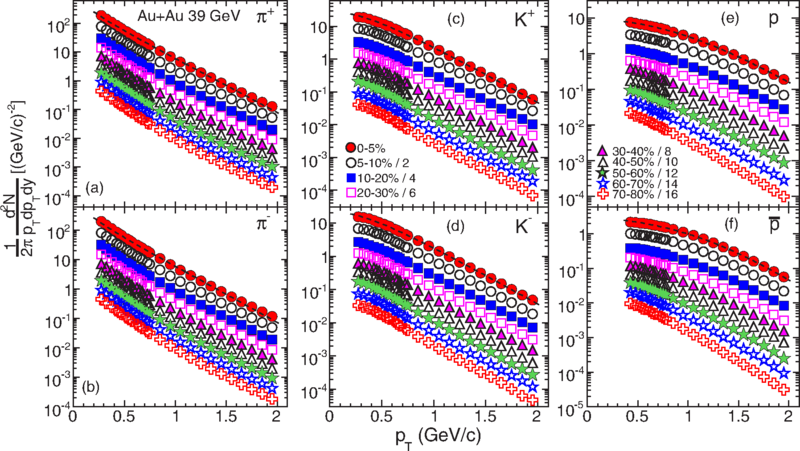
\includegraphics[width=6.5in]{../figures/PhysRevC-96-044904_pTSpectra_39.png}\\
  \caption{Transverse momentum spectra for $\pi^{+}$, $\pi^{-}$, $K^+$, $K^{-}$, $p$, and $\bar{p}$ at midrapidity ($|y|$ $<$ 0.1) from 39 GeV Au+Au collisions at RHIC. The fitting curves on the 0-5\% central collision spectra for pions, kaons, and protons/anti-protons represent, respectively, the Bose-Einstein, $m_{T}$-exponential, and double-exponential functions \cite{PhysRevC.96.044904}.}\label{fig:BESPaper_pTSpectra}
\end{figure}



\section{Extrapolation of Spectra}
The available spectra were limited to a range of transverse momenta from around 0.25 GeV/c to around 2 GeV/c (for pions). At higher momenta, with model-dependent values, the $p_{T}$ spectra may be dominated by hard-scattering processes. To account for the transverse energy corresponding to the momenta for which there were no available data, an extrapolation had to be used. The model used for the extrapolation and the associated statistics are discussed below.

\subsection{Boltzmann-Gibbs Blast Wave}
% https://arxiv.org/pdf/0812.1609.pdf
% https://arxiv.org/pdf/1703.02416.pdf
% 
The blast wave is a common model used in the analysis of particle momentum distributions \cite{Tang:2008ud,Tripathy:2017kwb,PhysRevC.96.044904}. The specific model used in this thesis is the Boltzmann-Gibbs blast wave (BGBW). This model assumes local thermal equilibrium at the kinetic freeze-out temperature for the applicability of a Boltzmann distribution. It also assumes a radially increasing velocity that attains a maximum value at the surface of the expanding fireball \cite{Tripathy:2017kwb}. The BGBW is represented by the equation: %It has the parameters mass, temperature, beta, v, and n. 

	\begin{equation}\label{eqn:BGBW}
	BGBW,
	\end{equation}
where $r$ is the radial distance from the collision vertex, $m$ is the particle mass, $T$ is the thermal freeze-out temperature, $\beta$ is the flow velocity, $\rho$ is the flow profile, $n$ is the flow velocity profile exponent, $K_{1}(x)$ and $I_{0}(x)$ are the modified Bessel functions given by...........................

% I assume that any anomalies in the magnitude of the normalization parameter do not affect the results significantly insomuch as they don't lead to: (a) unreasonable relative errors in the extrapolated values of the transverse energy, (b) any of the spectral fits having the extrapolated transverse energy more than that calculated from just the available spectra, and (c) for the 200 GeV collision samples, at least, the extrapolation at higher $p_{T}$ being more than that at lower $p_{T}$.


\subsection{Fitting Spectra to BGBW}
Figure \ref{fig:fit} presents an example of a BGBW fit on one of the individual particle spectra with $\chi^{2}$/ndf as well as other statistics and the associated uncertainties. The fitting is done in the ROOT software framework which is widely used in high energy physics data analysis. $T$, $\beta$, and $n$ are treated as free parameters, while $m$ is fixed. The results of the fits for each of the spectra are tabulated in appendix \ref{app:fitResults}
%A parallel-coordinates plot is presented in the next chapter in fig. \ref{fig:parallelCoord}, which shows the measured centralities, two of the good-fit parameters, and the calculated transverse energies for 270 different particles (lambdas not included).

	\begin{figure}[h]
	  \centering
	  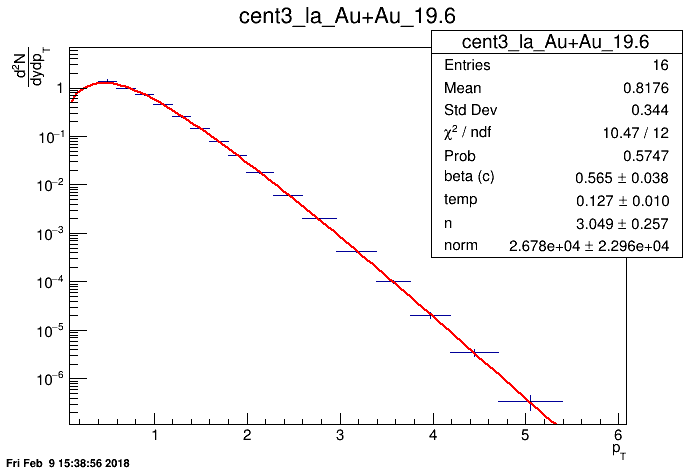
\includegraphics[width=4.5in]{figures/cent3_la_Au+Au_196.png}
	  \caption{Red curve shows the Boltzmann-Gibbs blast wave functional fit on the preliminary transverse momentum spectrum for lambda particles identified by the STAR detector for 19.6 GeV Au+Au collisions (10-15\% central). Parameters extracted from the chi-square goodness-of-fit test, as well as other statistics, are shown in the box on the top right.}\label{fig:fit}
	\end{figure}

\section{Calculations from the Spectra}
The available multiplicity distribution for the $p_{T}$ range, $p_{T,low}$ to $p_{T,high}$, of a spectrum divided the total spectrum into three different regions: $(i)$ region where the experimental data is available, i.e., $p_{T,low}$ to $p_{T,high}$, $(ii)$ extrapolation region from $p_{T}$ = 0 GeV/c to $p_{T}$ = $p_{T,low}$, and $(iii)$ extrapolation region from $p_{T}$ = $p_{T,high}$ to $p_{T}$ = 10 GeV/c,  
The total transverse energy and particle multiplicity for each of the spectra was calculated by adding said quantities corresponding to three different in the distribution.
\subsection{Calculation of $\frac{dE_{T}}{dy}$, $\frac{dE_{T}}{d\eta}$, $\frac{dN_{ch}}{dy}$, and $\frac{dN_{ch}}{d\eta}$}
The method described in section \ref{section:calcFromSpectra} +++++++++++++ talk about the jacobian from the appendix/previous chapter for conversion from y to eta was used to calculate ..........

.....corresponding to region $(i)$ was calculated by adding the areas of the rectangles corresponding to each $p_{T}$ bin.

\subsection{Corrections, Uncertainties, and Estimation of Total $E_{T}$}\label{corrections}
It is reasonable to assume that, at high energies, there should be roughly the same multiplicity of all the isospin states of a final state particle. This assumption was partially tested by comparing the $E_{T}$ values calculated for the identified charged particles with those independently calculated for their anti-particles for the same values of collision energy and centrality. The comparisons revealed the $E_{T}$ values of the particles being almost exactly equal to those of the antiparticles.

Table \ref{table:isospinStates} lists the isospin states associated with the pion, the kaon, the proton, and the lambda particles.
	\begin{table}[h!]
	\centering
	\begin{tabular}{|c c|}
	%\tabletypesize{\scriptsize}
	%\rotate
	\hline
	Particle & Isospin multiplets \\ [0.5ex]
	\hline
	\hline
	pion & $\pi^{+}, \pi^{0}, \pi^{-} $ \\
	kaon & $K^{+}, K^{0}, K^{-}, \bar{K}^{0}$ \\
	proton & $p, n, \bar{p}, \bar{n}$  \\
	lambda & $\Lambda, \bar{\Lambda}$  \\ [1ex]
	\hline
	\end{tabular}
	\caption{Isospin states of different identified particles.}
	\label{table:isospinStates}
	\end{table}
The total $E_{T}$ for all the particles would then be:	
	\begin{equation}\label{eqn:TotET}
	E_{T} = \frac{3}{2}(E_{T}^{\pi^{+}}+E_{T}^{\pi^{-}}) + 2(E_{T}^{K^{+}}+E_{T}^{K^{-}}) + 2(E_{T}^{p}+E_{T}^{\bar{p}}) + E_{T}^{\Lambda} + E_{T}^{\bar{\Lambda}}
	\end{equation}
	
 ................text content...................
 
\subsection{Lambdas Centralitiy Adjustments and $E_{T}$ Interpolations}
The centrality bins corresponding to the lambdas spectra were slightly different from those corresponding to the rest of the particles........
%\subsection{}
\section{Uncertainties}
.........The systematic uncertainties are assumed to be 100\% correlated point-to-point and uncorrelated between particles........ ?
%\section{}
